% =====================================================================
%  Page de garde — REMPLIR LES CHAMPS [BRACKETS]
% =====================================================================
\begin{titlepage}
  \centering
  \thispagestyle{empty}

  % ----- Bandeau supérieur : logos (gauche / milieu / droite) --------
  % Largeurs imposées (ratios très différents) ; \hfill répartit :
  % ensit1 collé à gauche, ensit2 au centre, ensit3 collé à droite.
  \noindent
  \makebox[\textwidth][s]{%
    
\includegraphics[height=2.4cm]{logos/ensit1.jpg}%
    \hfill
    
\includegraphics[height=2.4cm]{logos/ensit2.png}%
    \hfill
    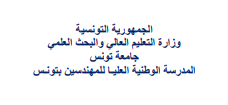
\includegraphics[height=2.4cm]{logos/ensit3.png}%
  }

  \vspace{1.0cm}

  % ----- Type de mémoire --------------------------------------------
  {\Large \textbf{Mémoire de fin d'études}\par}
  \vspace{0.3cm}
  {\large Présenté en vue de l'obtention du diplôme de\par}
  \vspace{0.2cm}
  {\large \textbf{Master en Data Science}\par}

  \vspace{1.5cm}

  % ----- Titre -------------------------------------------------------
  \rule{\linewidth}{0.6pt}
  \vspace{0.3cm}
  {\LARGE\bfseries
    Détection automatique de la fibrillation auriculaire\\
    à partir des intervalles RR\\
    par un réseau hybride CNN--LSTM\par}
  \vspace{0.3cm}
  \rule{\linewidth}{0.6pt}

  \vspace{1.5cm}

  % ----- Auteur ------------------------------------------------------
  {\large Réalisé par\par}
  \vspace{0.2cm}
  {\Large \textbf{Abdelmalek Abed}\par}

  \vspace{1.2cm}

  % ----- Encadrante & jury -------------------------------------------
  \begin{tabular}{ll}
    \textbf{Encadrante académique :} & Balkine Mansouri \\[4pt]
  \end{tabular}

  \vspace{0.6cm}

  \textbf{Membres du jury :}
  \begin{tabular}{ll}
    \phantom{} & \\
  \end{tabular}

  \vfill

  % ----- Année universitaire ----------------------------------------
  {\large \textbf{Année universitaire 2025--2026}\par}
\end{titlepage}
